\documentclass[12pt, letterpaper]{article}
\usepackage[titletoc,title]{appendix}
\usepackage{color}
\usepackage{booktabs}
\usepackage{caption}
\newcommand\fnote[1]{\captionsetup{font=small}\caption*{#1}}
\usepackage{float}
\usepackage[scaled=.7]{beramono}
\usepackage[usenames,dvipsnames,svgnames,table]{xcolor}
\definecolor{dark-red}{rgb}{0.75,0.10,0.10} 
\usepackage[margin=1in]{geometry}
\usepackage[linkcolor=blue,
            colorlinks=true,
            urlcolor=blue,
            pdfstartview={XYZ null null 1.00},
            pdfpagemode=UseNone,
            citecolor={blue},
            pdftitle={Not News}]{hyperref}

\usepackage{multibib}
\usepackage{geometry} % see geometry.pdf on how to lay out the page. There's lots.
\geometry{letterpaper}               % This is 8.5x11 paper. Options are a4paper or a5paper or other... 
\usepackage{graphicx}                % Handles inclusion of major graphics formats and allows use of 
\usepackage{amsfonts,amssymb,amsbsy}
\usepackage{amsxtra}
\usepackage{natbib}
\usepackage{longtable}
\usepackage{array}
\usepackage{multirow}
\usepackage{wrapfig}
\usepackage{colortbl}
\usepackage{pdflscape}
\usepackage{tabu}
\usepackage{threeparttable}
\usepackage{threeparttablex}
\usepackage[normalem]{ulem}
\usepackage{makecell}
\usepackage{verbatim}
\setcitestyle{round,semicolon,aysep={},yysep={;}}
\usepackage{setspace}             % Permits line spacing control. Options are \doublespacing, \onehalfspace
\usepackage{sectsty}             % Permits control of section header styles
\usepackage{lscape}
\usepackage{fancyhdr}             % Permits header customization. See header section below.
\usepackage{url}                 % Correctly formats URLs with the \url{} tag
\usepackage{fullpage}             %1-inch margins
\usepackage{multirow}
\usepackage{rotating}
\setlength{\parindent}{3em}
\usepackage{subcaption}
\usepackage{lmodern}
\usepackage[T1]{fontenc}
\usepackage{libertine}

\title{\Large{Hard News: Rise of Apolitical News in Network Television News}\footnote{Replication scripts and data are posted at: \url{https://github.com/notnews/notwork_news}.}}
\author{Gaurav Sood\thanks{Gaurav can be reached at \href{mailto:gsood07@gmail.com}{\footnotesize{\texttt{gsood07@gmail.com}}}}
\and Daniel Weitzel\thanks{Daniel can be reached at \href{mailto:daniel.weitzel@utexas.edu}{\footnotesize{\texttt{daniel.weitzel@utexas.edu}}}}}

\date{\vspace{.5cm}\normalsize{\today}}

\begin{document}
\maketitle

\begin{comment}

setwd(paste0(githubdir, "notwork_news/ms"))
tools::texi2dvi("us_news.tex", pdf = TRUE, clean = TRUE) 
setwd(basedir)

\end{comment}

\begin{abstract}
Network television news is among the most frequently consumed news in the country. But there is little data on what is covered on network news. Or how the quality of network news has fared over the years. We exploit the Vanderbilt Television News Archive, the largest publicly available database of TV news, to learn about two important aspects of the production of news: geographic focus and political content. Using data from a random sample of over 5,000 broadcast segments spanning 1968--2019, we find that the percentage of network television news devoted to topics unrelated to politics steadily increased from less than 5\% in 1968 to over 10\% in the last 15 years. The pattern of change in geographic focus is more complex, but there is a clear rise in the percentage of local news over the last two decades. The percentage of local news increased from about 5\% in 2000 to over 25\% in 2019.
\end{abstract}

\clearpage
\doublespacing
Network television news is among the most frequently consumed news in the country \citep{pew2019, pew2020}. But there is little data on what is covered on the network news or how the coverage has changed over the years. We exploit data from Vanderbilt Television News Archive (VTNA), the largest publicly available database of TV news, to shed light on two important aspects of the quality of news: geographic focus (local, national, and international) and political relevance (whether or not the news is about a politically relevant topic) \citep{curran2009media}. Coding a random sample of over 5,000 broadcast segments spanning 1968--2019, we find that the percentage of network television news devoted to topics unrelated to politics steadily increased from less than 5\% in 1968 to over 10\% in the last 15 years. The pattern of change in geographic focus is more complex, but there is a clear rise in the percentage of local news over the last two decades. The percentage of local news increased from about 5\% in 2000 to over 25\% in 2019.

\section*{Data and Measurement}
VTNA contains a continuous collection of the daily news broadcasts from \emph{ABC}, \emph{CBS} and \emph{NBC} since 1968. A few news shows from \emph{CNN} and \emph{Fox News} are available starting 1995 and 2004, respectively. In total, the archive has over 1M broadcast abstracts from US network channels between 1968 and 2019 \citep{lynch1996vanderbilt, soodlaohaprapanon2020}. For each segment of a news broadcast, the data includes information on the channel, broadcast date, duration, program title, and an abstract of the content of the segment (see Figure \ref{fig:vandy_abstract}). 

\begin{figure}[H]
  \centering
  \caption{Example of VTNA broadcast segment abstract. CBS Evening News segment from Feb 01, 2001}
  \label{fig:vandy_abstract}
  
\includegraphics[width=.8\linewidth]{../figs/fig_vtna_screenshot_4.png}
\end{figure}

We limit our focus to the three main networks: ABC, NBC, and CBS. Figure \ref{fig:vandy_channel} shows the total number of news broadcasts with abstracts available for the three network channels between 1968 and 2019. The number of news segments from CBS and NBC falls sharply, starting in 2015.

From this data, we randomly sampled 100 stories from each year between 1968 and 2019. We weighted the sample by broadcast duration so that we have a random sample of content broadcasted in time. The sampled abstracts for 1968 to 1977 accidentally included news specials. We removed those posthoc. In all, we sampled 5,200 stories. The three network news channels make up 3,928 broadcast abstracts in the sample (ABC--1,374, CBS--1,228, and NBC--1,326). (The remaining abstracts were from news shows on other channels, such as CNN and Fox News.)

\begin{figure}[H]
  \centering
  \caption{News Broadcasts by Channel in VTNA}
  \label{fig:vandy_channel}
  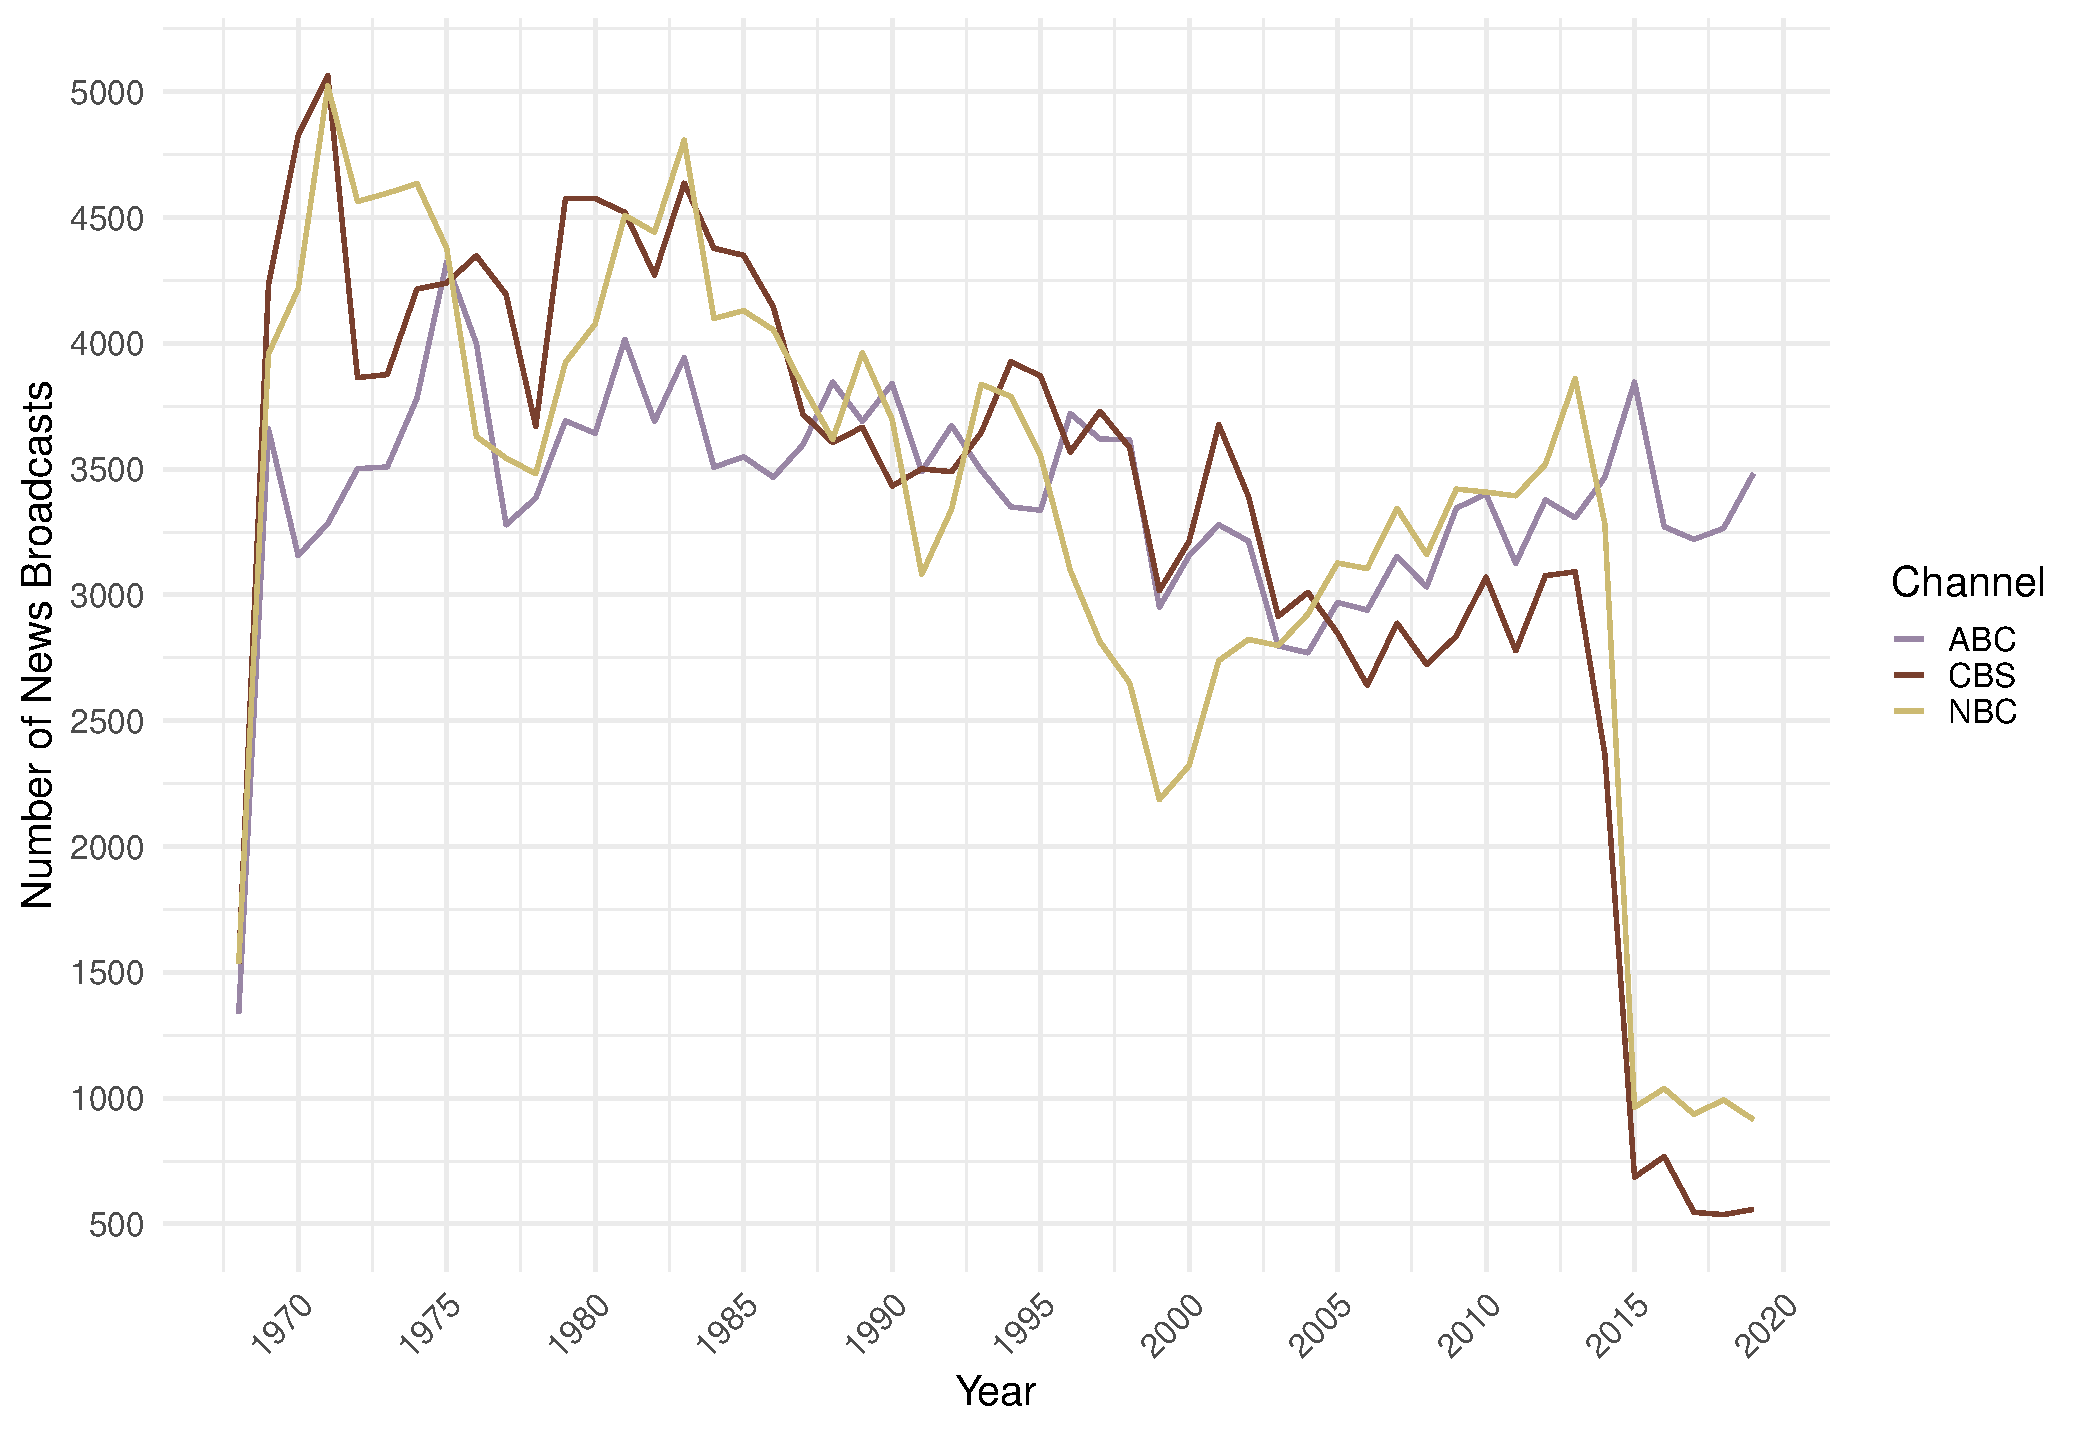
\includegraphics[width=.95\linewidth]{../figs/fig_channel_total.pdf}
\end{figure}

We coded the abstracts of the news segments for geographic scope (local, national, international) and news type (soft vs. hard news). (See \ref{appendix:coding_scheme} for coding scheme and \ref{appendix:screenshots} for screenshots of the coding scheme, examples, instructions, and a sample question with the instrument.) By soft news, we mean ``information that is either personally useful or merely entertaining'' \citep{zaller2003new}.\footnote{By soft news, we mean the precise content of the news as opposed to ``soft news media''---shows that primarily carry soft news but sometimes carry hard news (e.g., \cite{baum2006oprah}).}

We crowdsourced the coding of these abstracts using \textit{Figure Eight} (now \textit{Appen}). We crowdsourced the coding of these abstracts using \textit{Figure Eight} (now \textit{Appen}). Three different coders coded each broadcast abstract. The number of news abstracts coded by a coder ranges between 12 and 347. The mean is 56.6, and the standard deviation is 49. 

To guarantee high-quality coding, we coded 230 randomly chosen questions ourselves and included those as gold standard questions in the survey.\footnote{The list of gold standard questions and their answers is available \href{https://github.com/notnews/notwork_news/blob/master/data/sample_questions_gold.csv}{here (CSV)}.} The fewest gold standard questions that a coder had to field was 9. Any answer from a coder who answered less than 80\% on the gold standard questions was replaced by an answer from a coder who got 80\% or more of the gold standard questions correct. The average score on gold standard questions for the type of news and geographic focus was 88.1\% and 88.6\%, respectively. 

The inter-coder agreement among coders who met the standard for geographic scope was 50.1\%, and news classification was 80.3\%. Krippendorf's $\alpha$ for the tasks for 0.4 and 0.3, respectively. 

For our main results, we subset our analysis to stories where two or more of the high accuracy coders agreed on the label. For the type of news, this means sacrificing ten rows, and for the geographic focus, it means sacrificing 195 rows or less than 5\% of the data. And we assign the story the label given by the majority.

\section*{Results}
Network news is steadily becoming softer (see Figure \ref{fig:soft_over_time}). From less than 5\% in the late 1960s and early 1970s, the percentage of soft news is more than 10\% in the last 15 or so years. There is little difference across channels, in means as well as slope. As Table \ref{tab:news_over_time} shows, the potential maximum mean difference between ABC, CBS, and NBC is about 2\%. We do not have enough data to estimate slope over time within channels, but whatever data we have suggests the differences are non-existent (see Figure \ref{fig:soft_over_time_by_channel}). Limiting inference to years where we have consistent data (1970--2014) doesn't affect the results (see Table \ref{tab:news_over_time_7014}).

\begin{figure}[H]
  \centering
  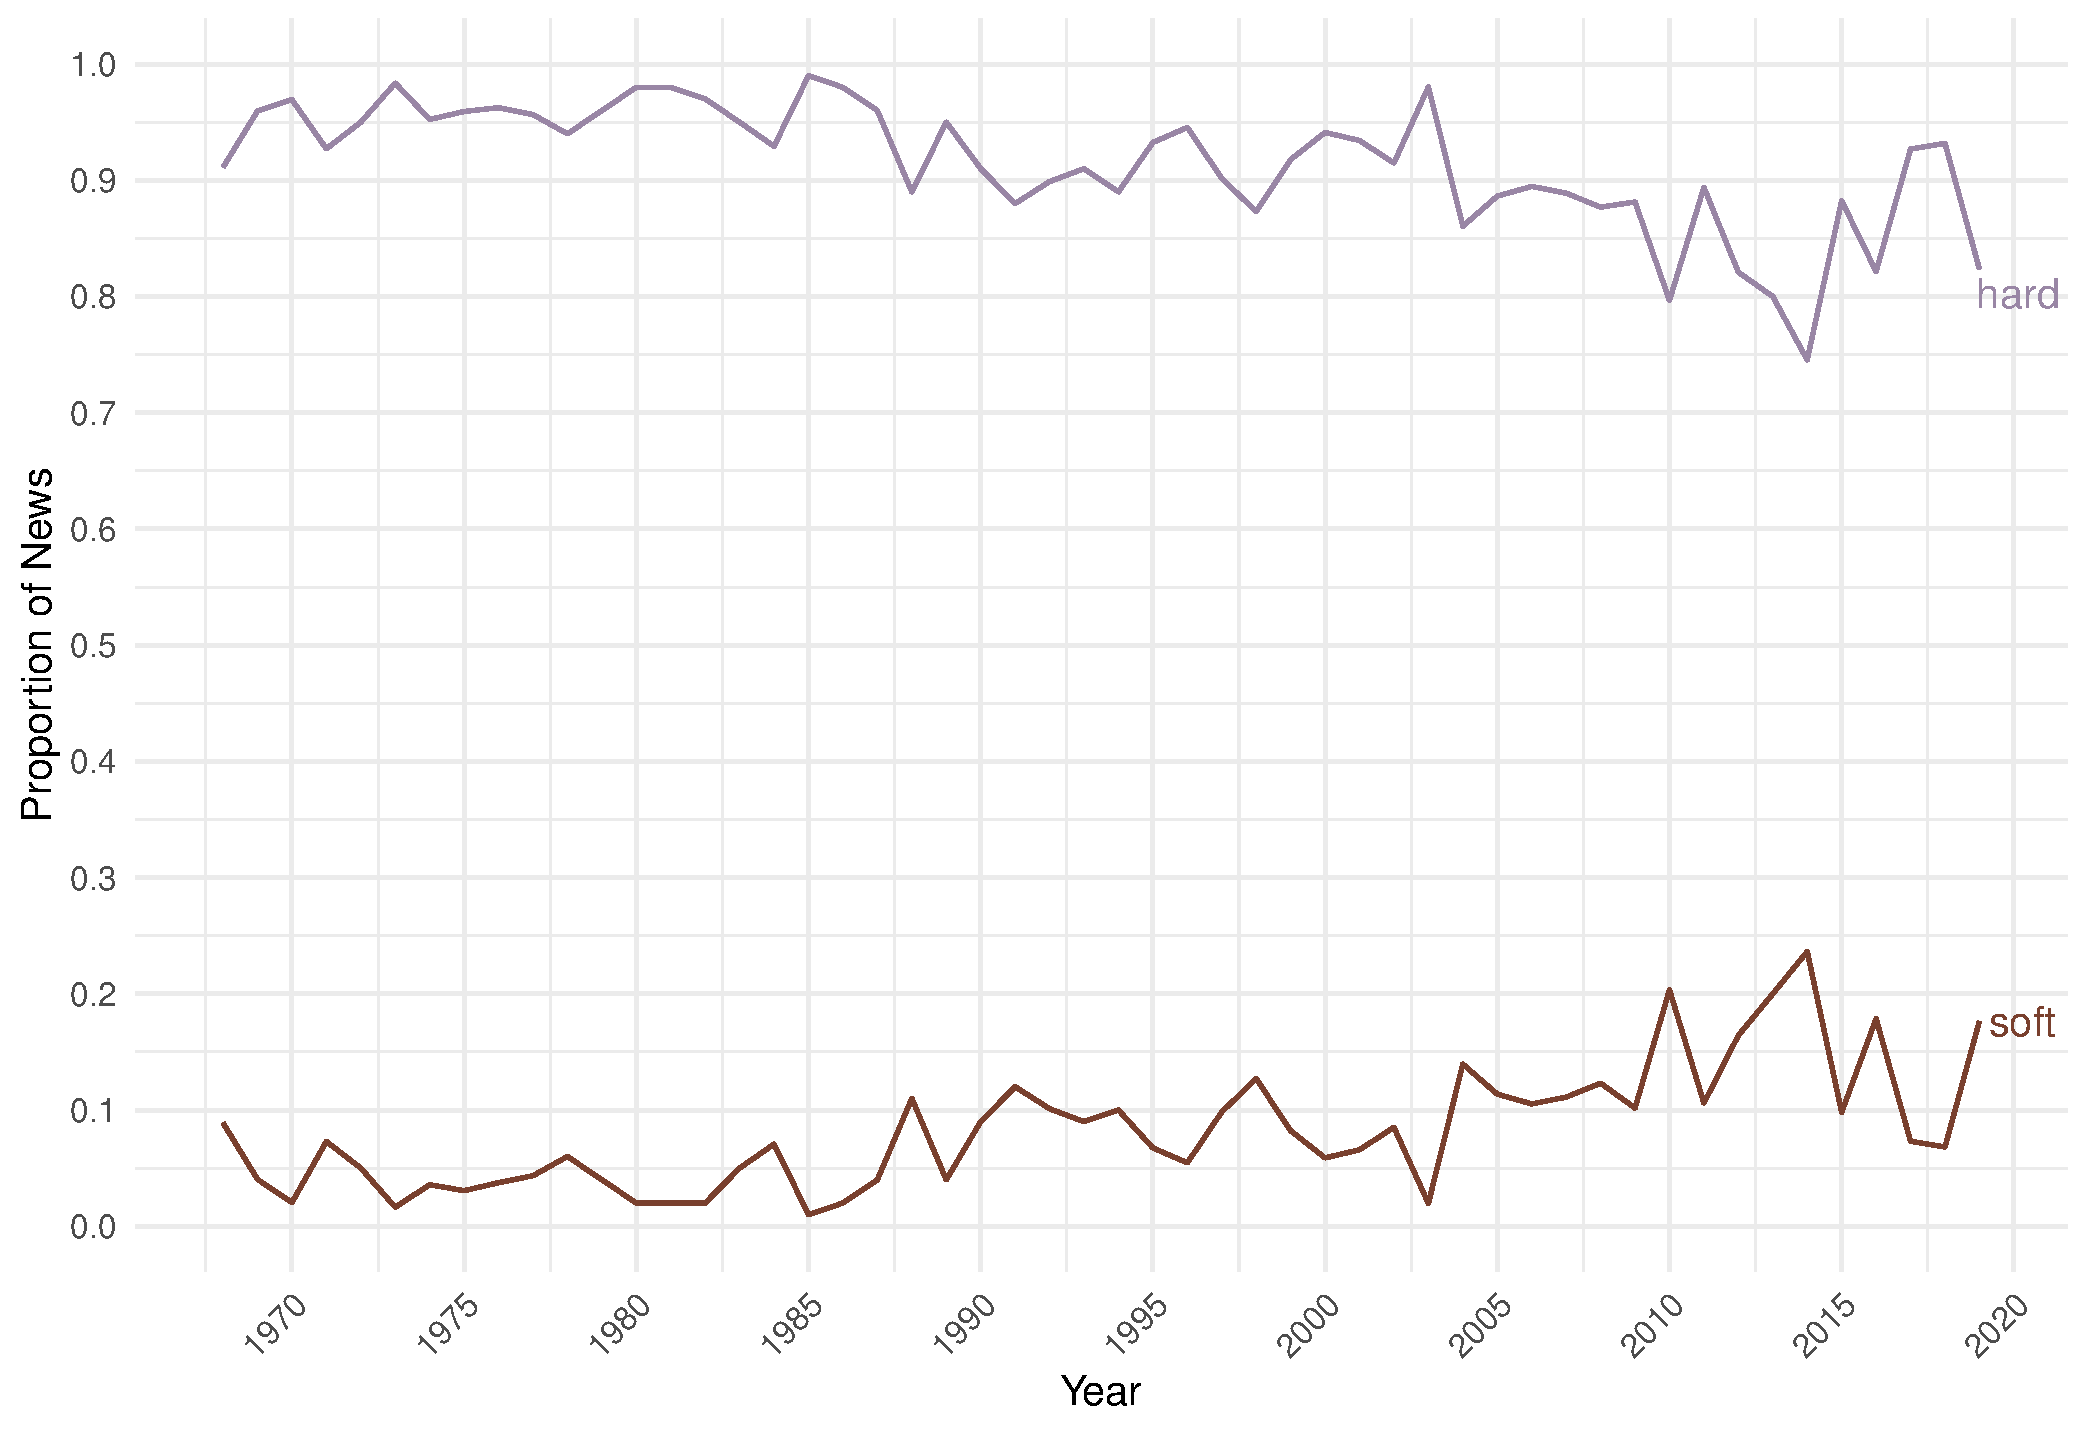
\includegraphics[width=.95\linewidth]{../figs/fig_prob_news_all.pdf}
  \caption{Proportion of Hard and Soft News Over the Years}
  \label{fig:soft_over_time}
\end{figure}


\begin{table}
\caption{Explaining The Provision of Different Types of News by Channel and Year}
\begin{center}
\begin{tabular}{l c c c c }
\hline
 & Soft & International & National & Local \\
\hline
(Intercept)  & $0.08^{***}$ & $0.31^{***}$ & $0.59^{***}$  & $0.10^{***}$ \\
             & $(0.01)$     & $(0.01)$     & $(0.01)$      & $(0.01)$     \\
Channel: CBS & $-0.01$      & $-0.02$      & $0.03$        & $-0.01$      \\
             & $(0.01)$     & $(0.02)$     & $(0.02)$      & $(0.01)$     \\
Channel: NBC & $-0.01$      & $0.02$       & $-0.02$       & $-0.00$      \\
             & $(0.01)$     & $(0.02)$     & $(0.02)$      & $(0.01)$     \\
Year         & $0.04^{***}$ & $-0.00$      & $-0.05^{***}$ & $0.05^{***}$ \\
             & $(0.00)$     & $(0.01)$     & $(0.01)$      & $(0.00)$     \\
\hline
R$^2$        & 0.02         & 0.00         & 0.01          & 0.03         \\
Num. obs.    & 3923         & 3733         & 3733          & 3733         \\
\hline
\multicolumn{5}{l}{\scriptsize{$^{***}p<0.001$, $^{**}p<0.01$, $^*p<0.05$}}
\end{tabular}
\label{tab:news_over_time}
\end{center}
\end{table}


Moving to the geographic focus of news, the pattern in local news is the clearest. Since the 2000s, the provision of local news has increased substantially. It has moved from roughly 5\% to 20\% (see Figure \ref{fig:sub1_over_time}). Between 1985 and 2000, there was another concave curve peaking in the early 1990s at about 20\%. Between 1970 and 1985, the provision remains flat. 

Percentages of national and international news seem to follow a pattern with national news generally peaking around presidential elections (see Figure \citep{fig:national_president}) and international news peaks during wars (see Figure \ref{fig:international_war}).

\begin{figure}[H]
  \centering
  \caption{Proportion of Local, National, and International News Over the Years}
  \label{fig:sub1_over_time}
  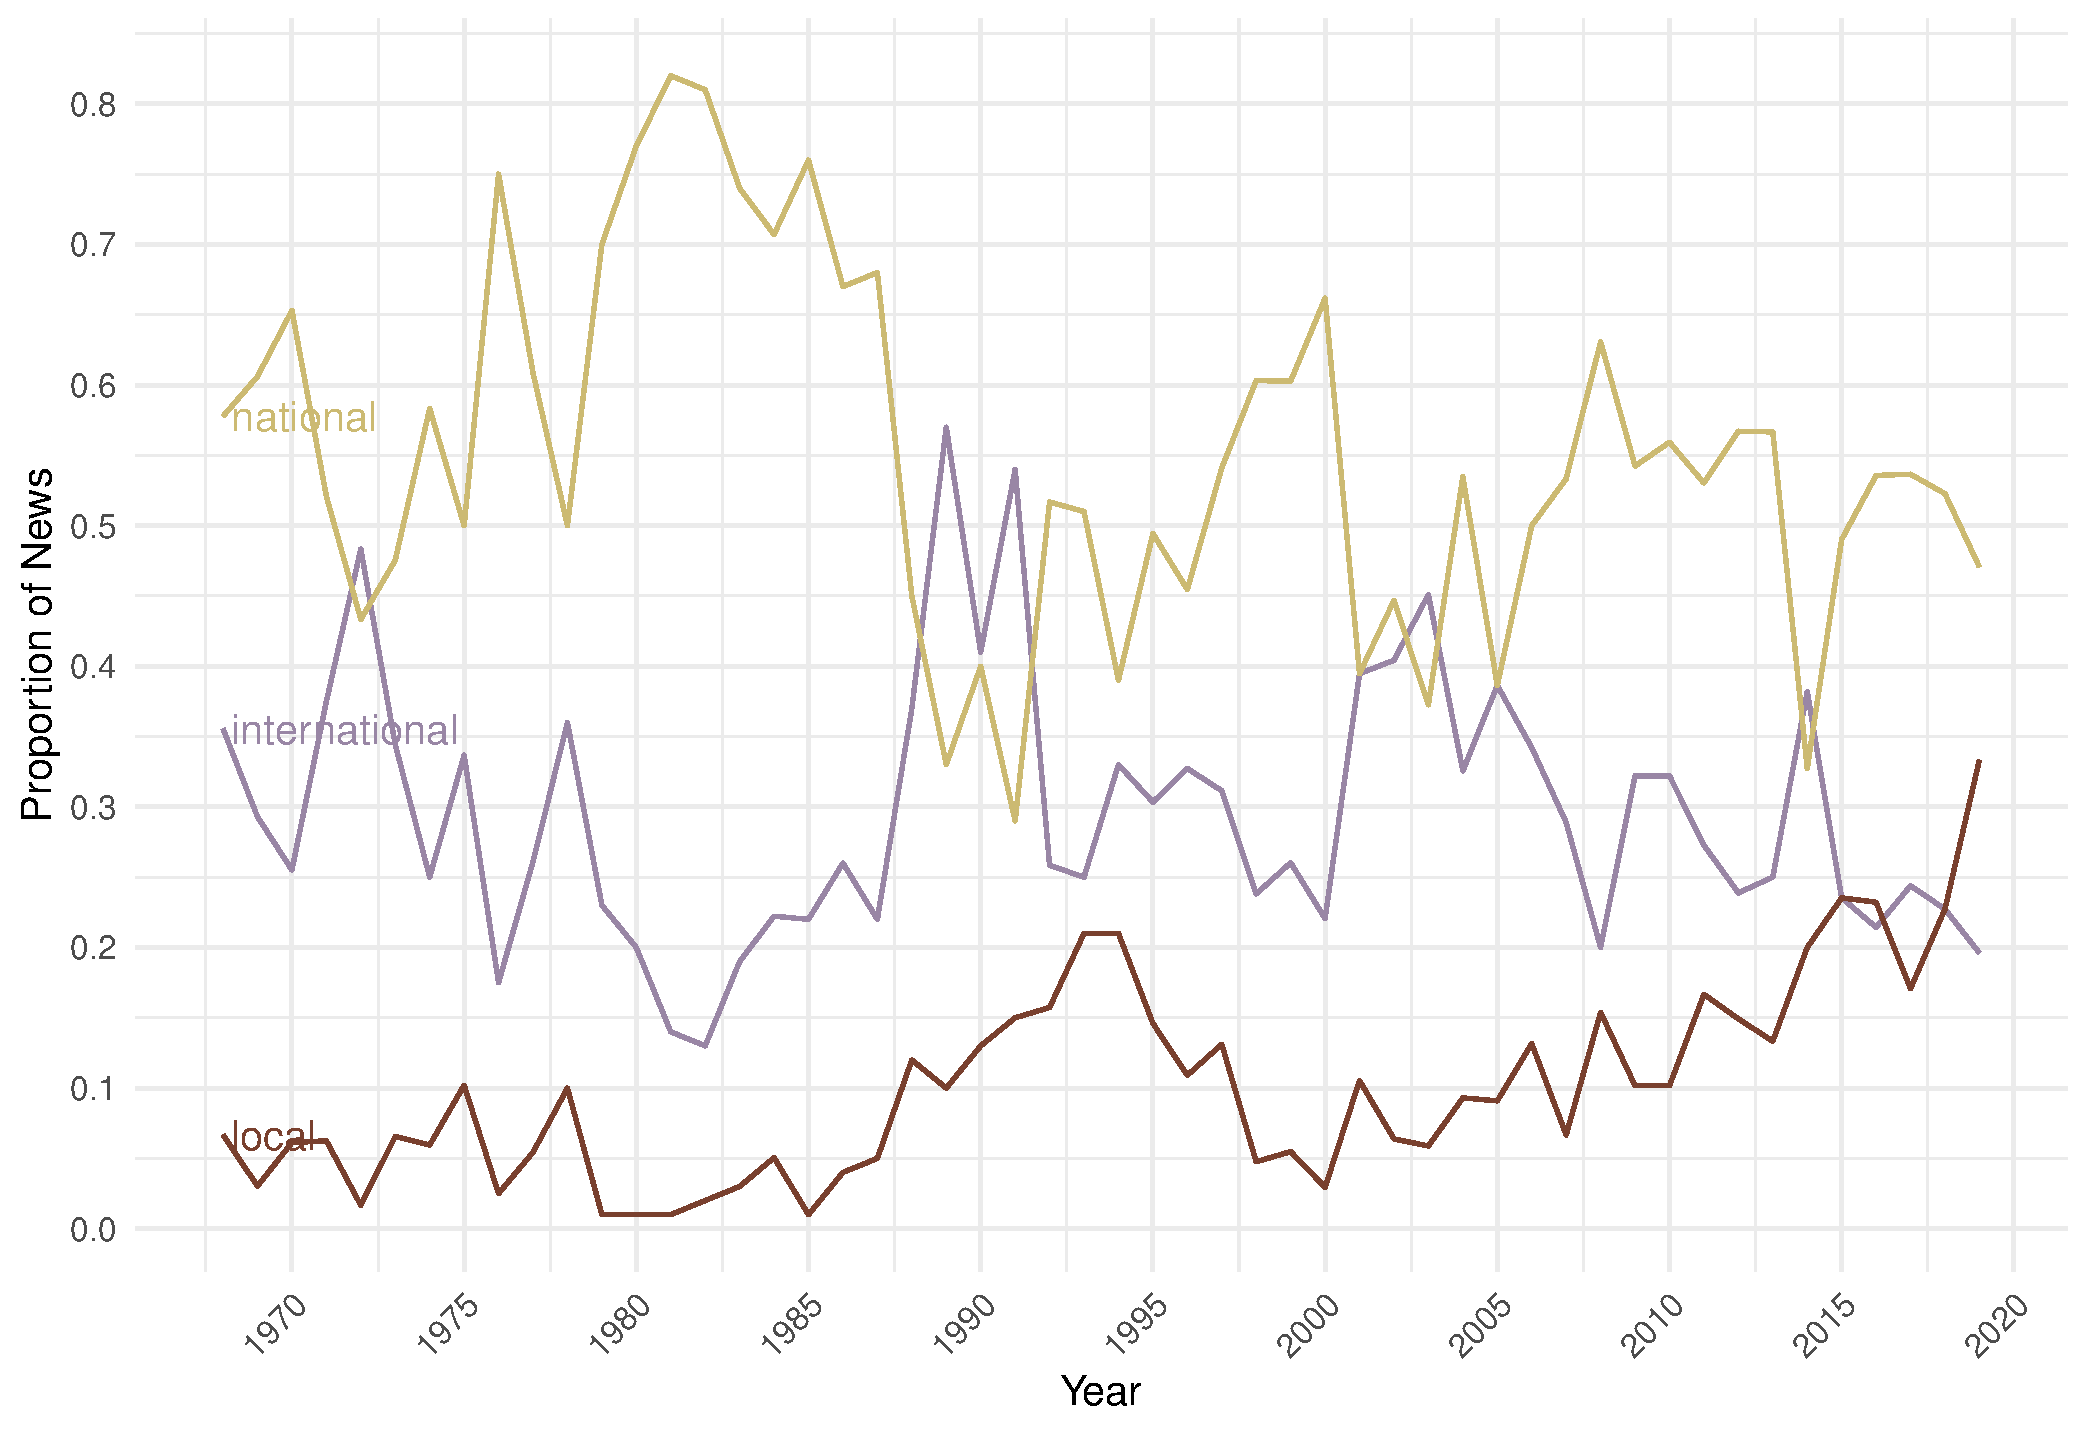
\includegraphics[width=.95\linewidth]{../figs/fig_geography.pdf}
\end{figure}

\begin{figure}[H]
  \centering
  \caption{International News and Key International Events}
  \label{fig:international_war}
  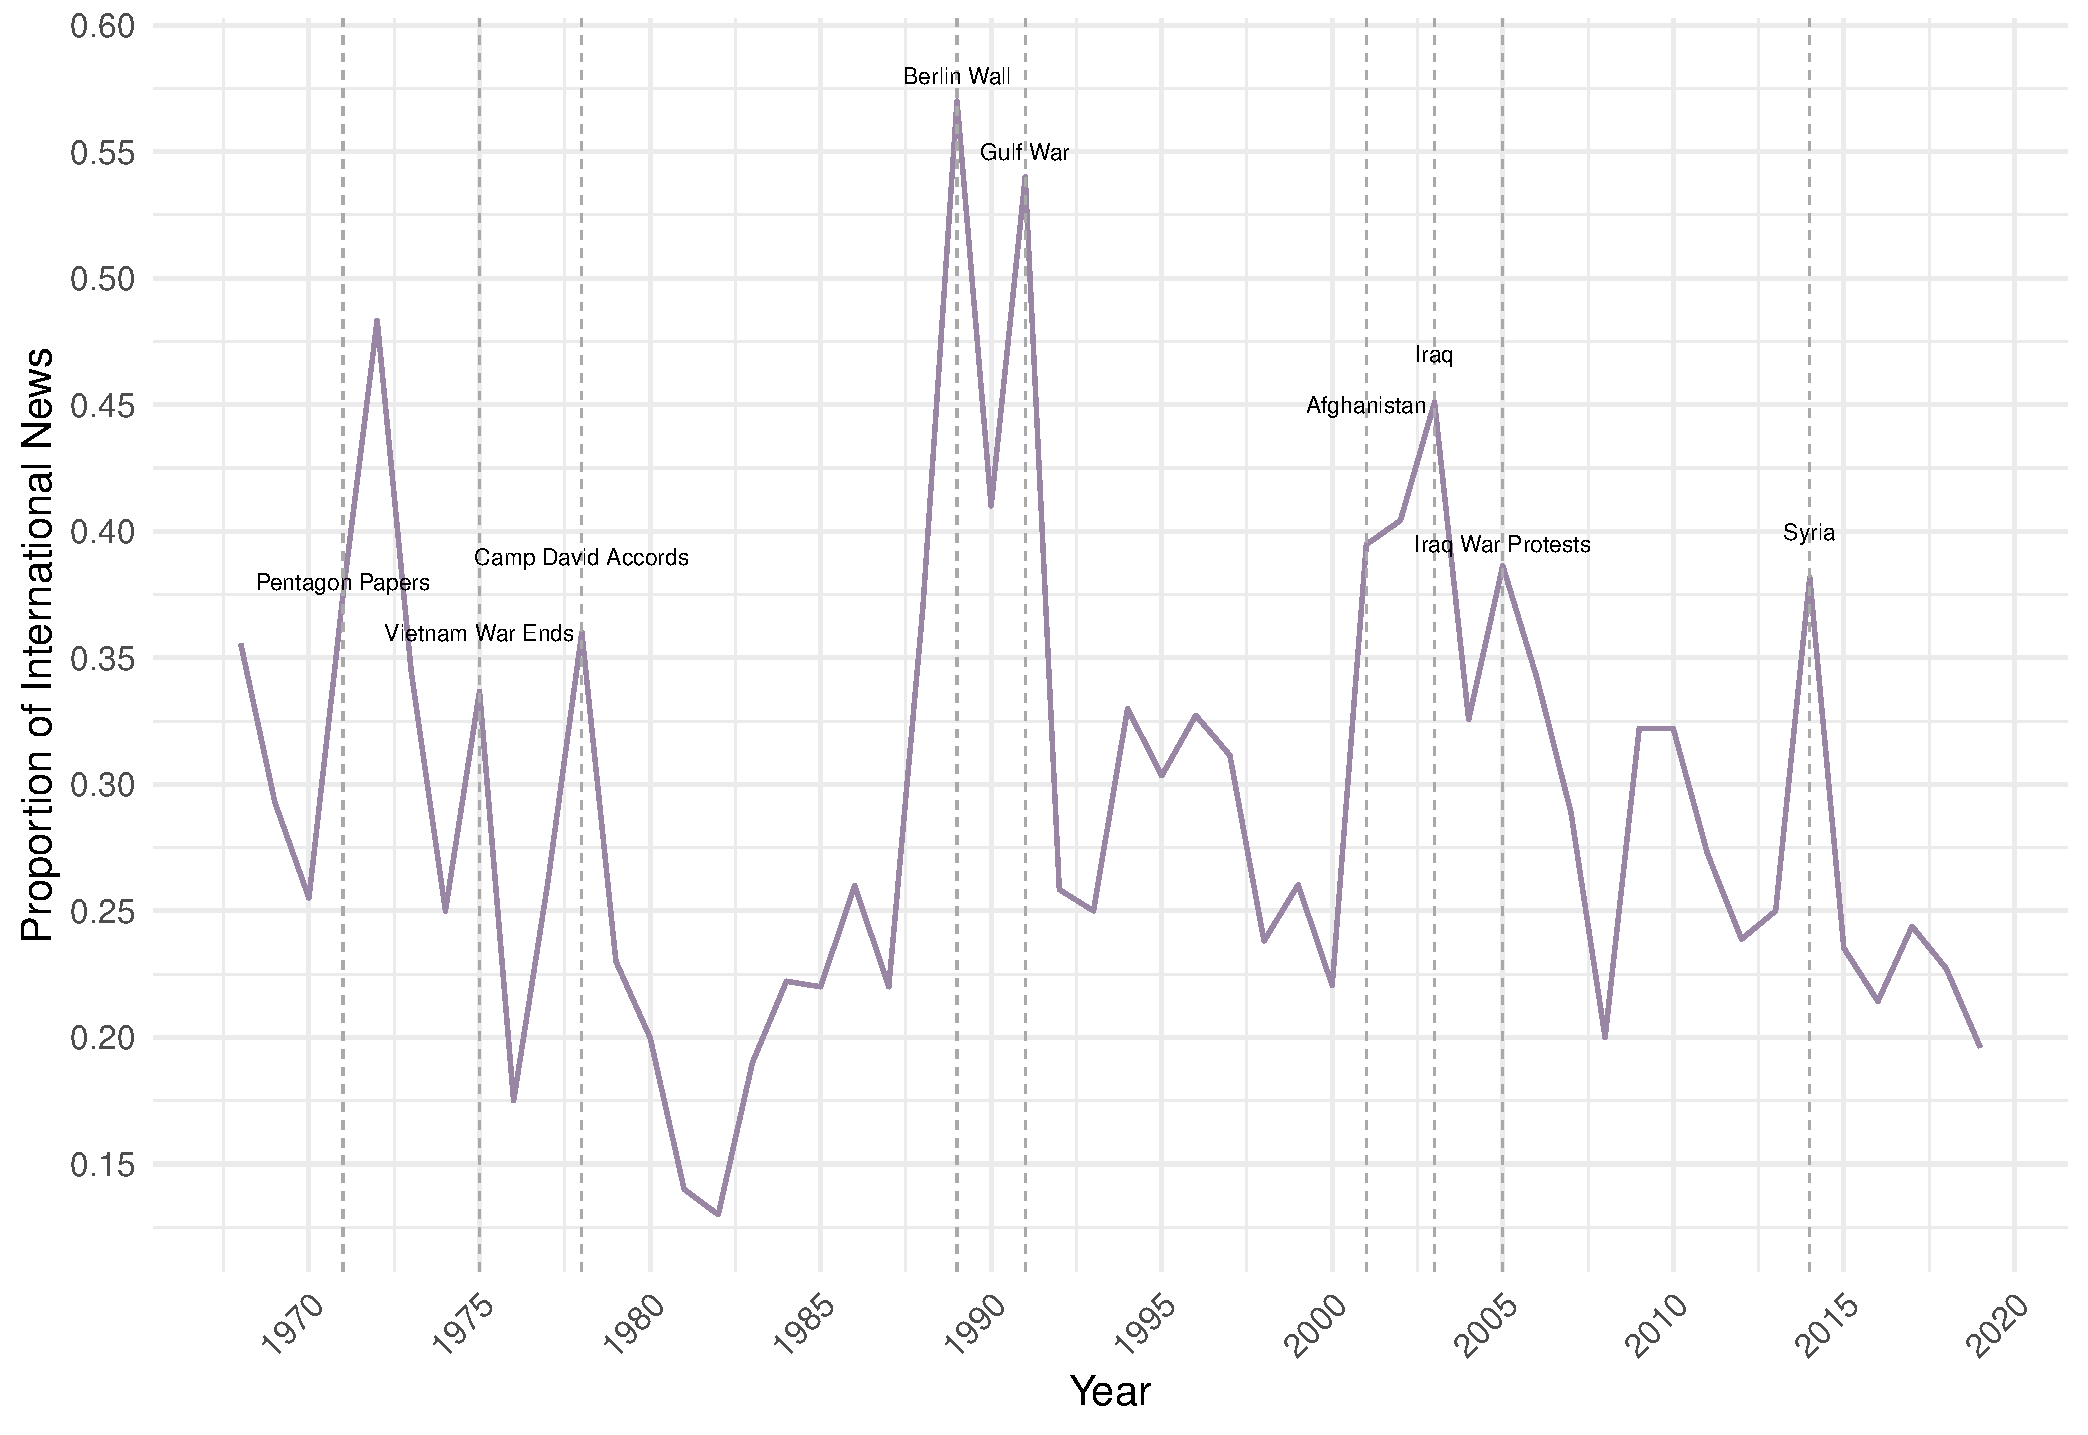
\includegraphics[width=.95\linewidth]{../figs/fig_geography_wars.pdf}
\end{figure}

\begin{figure}[H]
  \centering
  \caption{National News and Presidential Elections}
  \label{fig:national_president}
  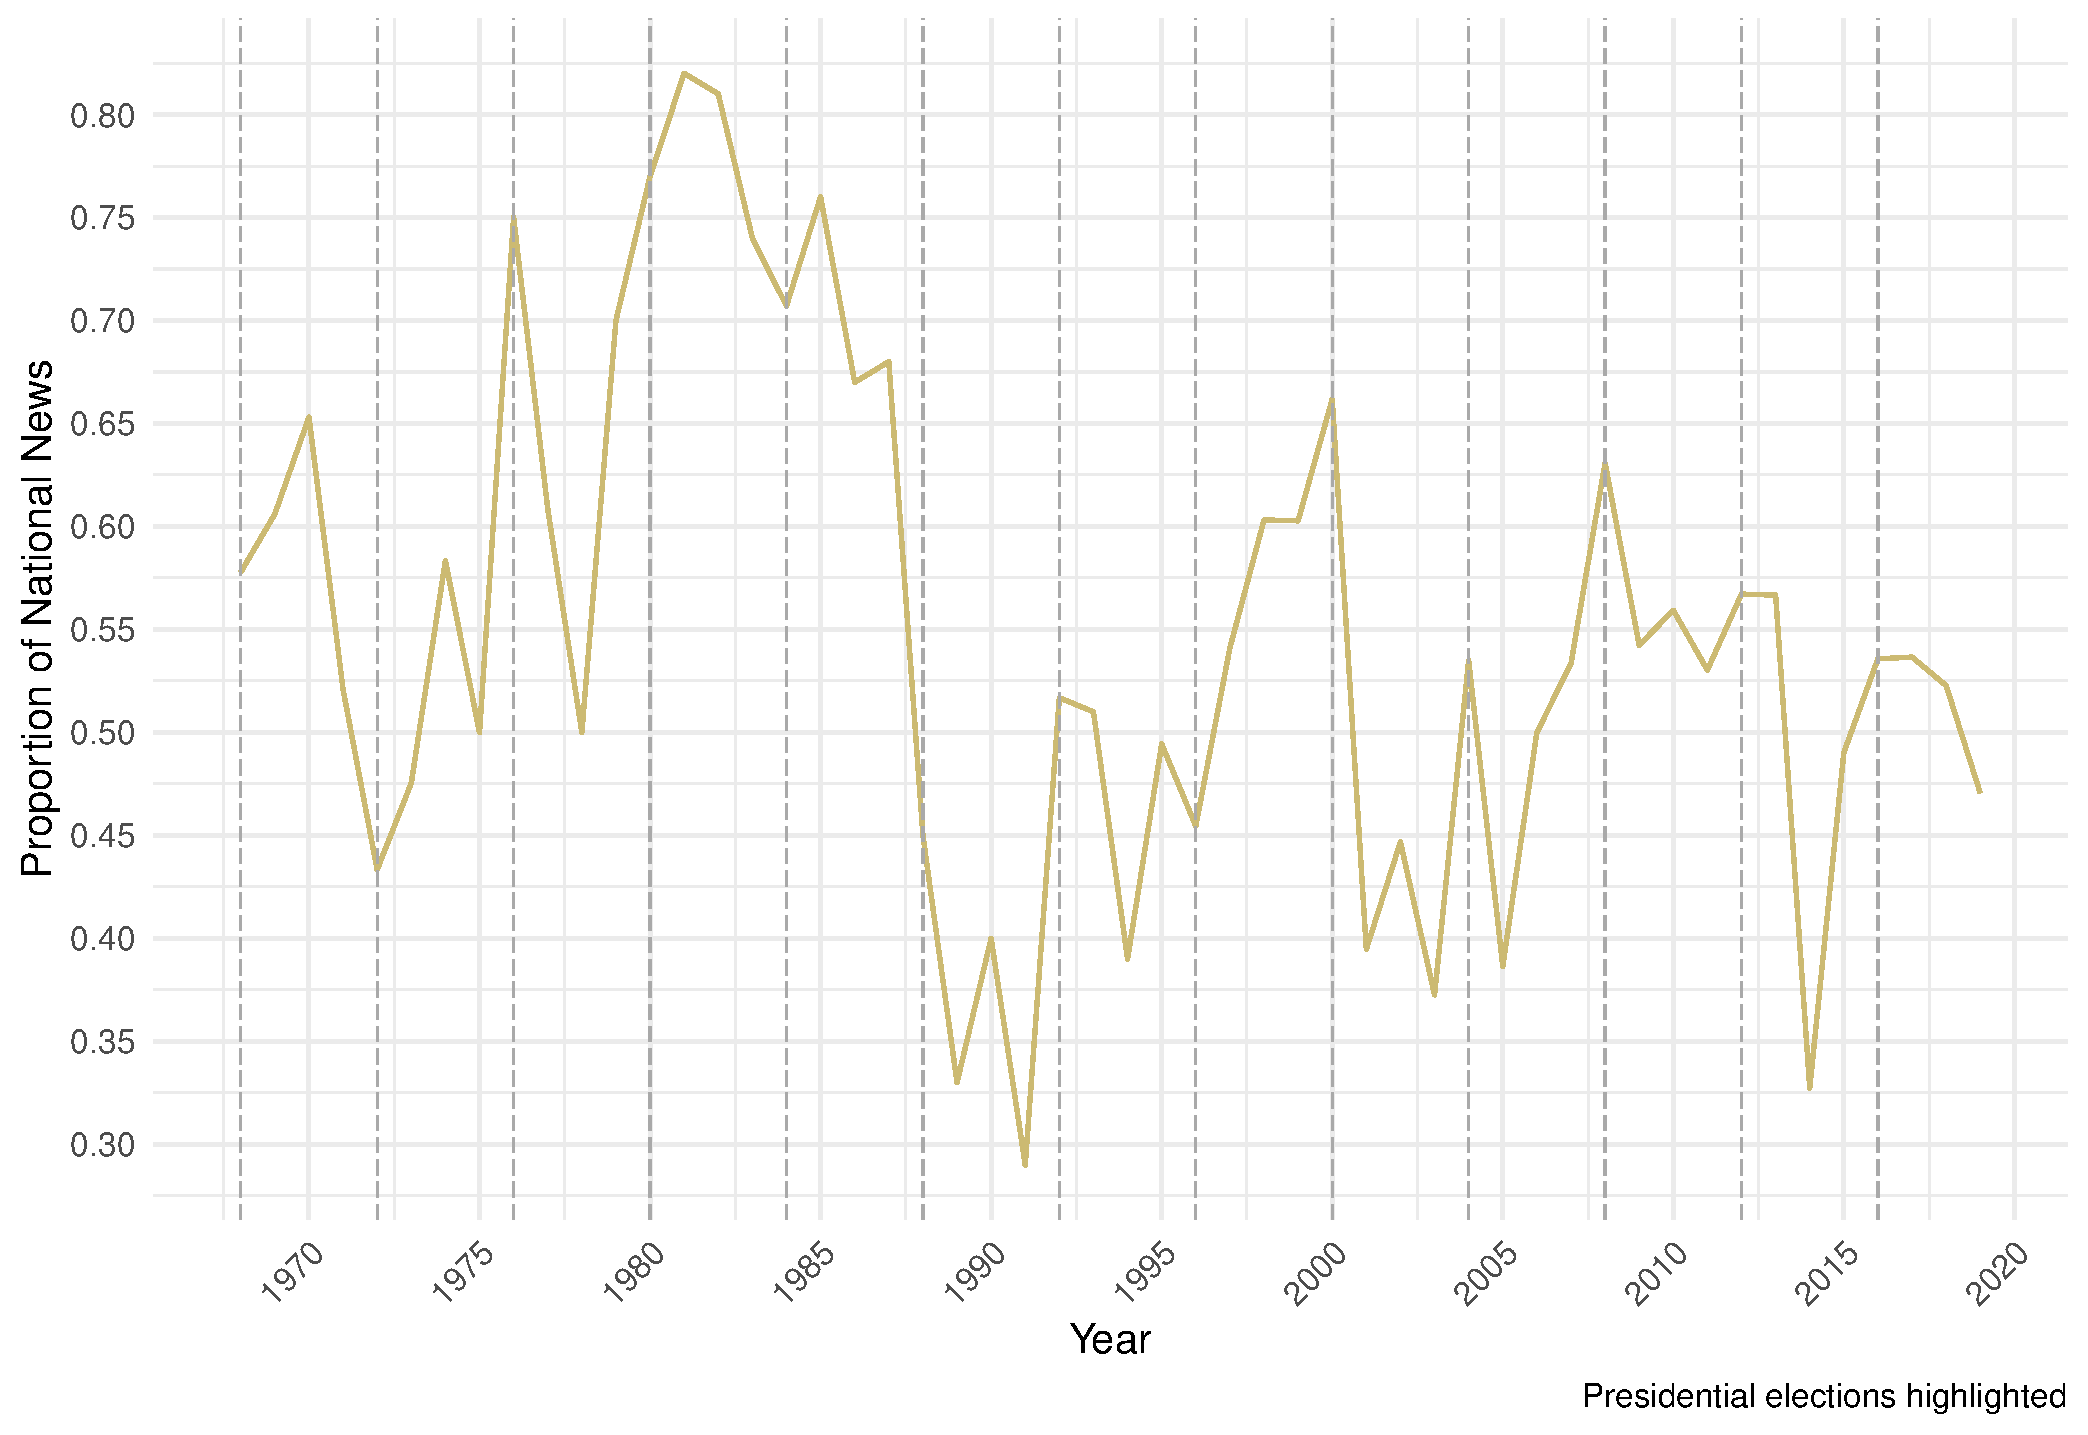
\includegraphics[width=.95\linewidth]{../figs/fig_geography_presidential.pdf}
\end{figure}

Our numbers are sharply different from those obtained by \cite{curran2009media}. In the media analysis by Curran et al., in 2007, about 27\% of the television news was soft. Our numbers are closer to 10\%. For geographic focus, our numbers are closer to 30\% while the Curran et al. estimate is 20\%. 

\section*{Discussion}
Network television news was widely regarded for its quality in the 1960s and 1970s \citep{hallin1990whatever}. Was the esteem it was held in deserved? And how has the quality fared since? These questions have added urgency given network television news continues to be among the most common sources of news for Americans. Capitalizing on a vast dataset of news transcripts, we have an answer. The quality of news has declined somewhat, with soft news constituting twice as large a share today than 70 years ago. 

\clearpage
\bibliographystyle{apsr}
\bibliography{us_news}  

\clearpage
\appendix
\renewcommand{\thesection}{SI \arabic{section}}
\renewcommand\thetable{\thesection.\arabic{table}}  
\renewcommand\thefigure{\thesection.\arabic{figure}}
\counterwithin{figure}{section}

\section{Supporting Information}

\subsection{Coding Scheme}
\label{appendix:coding_scheme}

You will see snippets of stories from American television news. We would like to classify these snippets on the following two dimensions:

\begin{itemize}

    \item    Soft or Hard News:
        \begin{itemize}
            \item Soft News: News about topics like:
            \begin{itemize}
                \item Sports
                \item Weather (but not climate, e.g., global warming is excluded)
                \item Entertainment celebrities 
                \item Travel
                \item Style/Fashion
                \item Cooking
                \item Arts or Literature
                \item Personal Tech.: New Apple products, etc.
                \item Personal health: How to sleep better, etc. 
            \end{itemize}
    
            \item Hard News: News that is politically consequential. News that tells us the state of the world, e.g., unemployment, crime, poll results, etc. or news that talks about policies being debated, e.g., healthcare bill, abortion bill, Medicare, Medicaid, etc. Among others, it includes the following areas:
            \begin{itemize}
                \item Politicians, Parties, Elections, and Polling: Poll results, candidate profiles, election results, etc.
                \item Economy: Taxes, Inflation, Unemployment, Trade, GDP, etc.
                \item Education: Educational policies, schools, universities, students, educational budgets, etc.
                \item Environment: Environmental policies and protection, global warming, plastics, pollution, etc. 
                \item Justice System, Law and Order, Crime: Crime rates, incarceration, news of specific crime, etc.
                \item Terrorism, War, Conflict, Military
                \item Immigration/Asylum
                \item Morality, Family Values, Religion: Abortion, homosexuality, etc.
                \item Public Health: New drug discoveries, food recalls, vaccines, etc.
                \item Social Welfare: Medicare, Medicaid, Public Housing, Anti-poverty
                \item Health Insurance
                \item Other Policy Areas: Agriculture and Rural Affairs, Child Care, and Family Policies
            \end{itemize}
        \item Clarifying Differences Between \textbf{Hard} and \textbf{Soft News}:
            \begin{itemize}
                \item \textbf{Hard News}: News that is politically consequential, e.g., news about the state of the world, e.g., unemployment numbers, crime, terrorist attack, poll results, etc., news about policies being debated, e.g., healthcare, abortion, immigration, civil rights, Medicare, etc.
                \item  \textbf{Soft News}: News about personal technology, e.g., new iPhone, etc., cooking, sports, style, fashion, music, arts, literature, etc.
            \end{itemize}

            \begin{itemize}
                \item    Technology
                    \begin{itemize}
                        \item News about personal tech. like latest Apple products are \textbf{Soft News}
                        \item News about new technologies like advancement in semiconductors, energy, space exploration is \textbf{Hard News}.
                    \end{itemize}
                \item Weather
                    \begin{itemize}
                        \item News about how the weather will be, etc., is \textbf{Soft News}
                        \item News about climate change, global warming, flooding, etc. is \textbf{Hard News}
                    \end{itemize}

                \item    Health:
                    \begin{itemize}
                        \item News about personal well being like tips for sleeping and eating better is \textbf{Soft News}
                        \item News about new nutrition guidelines, drug discoveries, food recalls, etc. is \textbf{Hard News}
                    \end{itemize}
            \end{itemize}
        \end{itemize}
    \item Geography:
        \begin{itemize}
            \item Local — deals with a village, city, town, or state.
            \item National — deals with more than one state or the country as a whole
            \item International — deals with international issues.
        \end{itemize}
\end{itemize}

\clearpage
\subsection{Screenshots of the Coding Scheme, Examples, Instructions, and Sample Question With Instrument}
\label{appendix:screenshots}

\begin{figure}[H]
  \centering
  \caption{Coding Scheme}
  \label{fig:coding_scheme}
  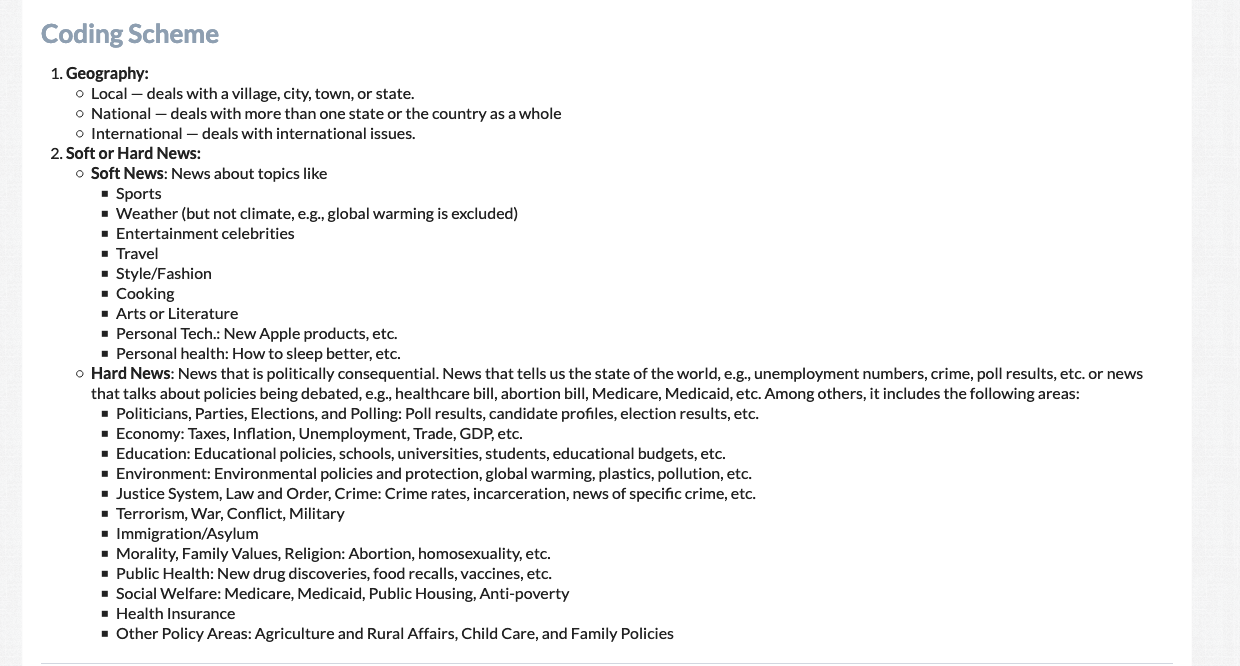
\includegraphics[width=\linewidth]{../data/screenshots/coding_scheme.png}
\end{figure}

\begin{figure}[H]
  \centering
  \caption{Clarifying Differences Between Hard and Soft News}
  \label{fig:clarifying_diff}
  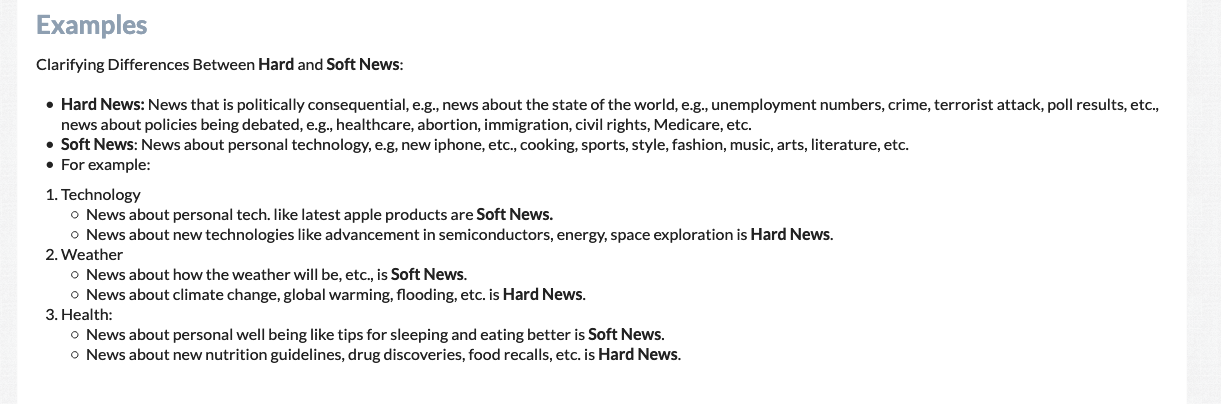
\includegraphics[width=\linewidth]{../data/screenshots/clarifying_diff.png}
\end{figure}

\begin{figure}[H]
  \centering
  \caption{Examples}
  \label{fig:examples}
  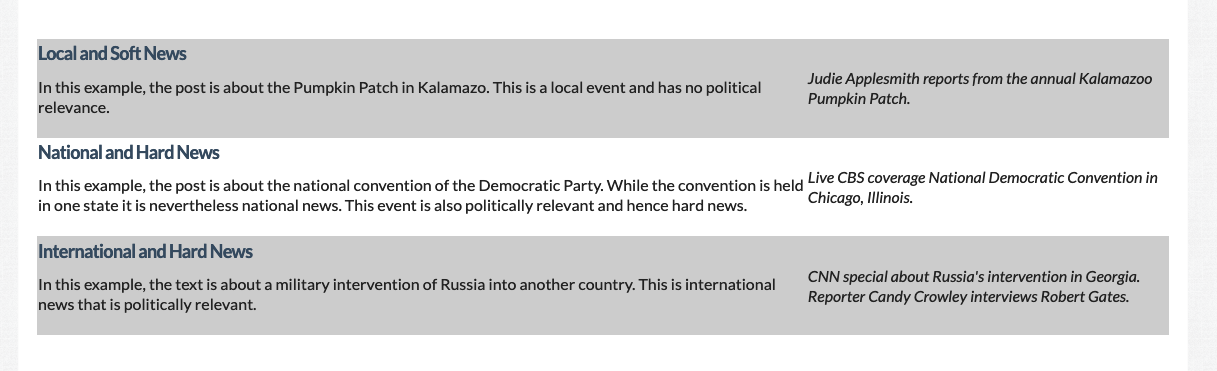
\includegraphics[width=\linewidth]{../data/screenshots/examples.png}
\end{figure}

\begin{figure}[H]
    \centering
    \caption{Instructions}
    \label{fig:instructions}
    
\includegraphics[width=\linewidth]{../data/screenshots/instructions.png}
\end{figure}

\begin{figure}[H]
  \centering
  \caption{Sample Question}
  \label{fig:test}
  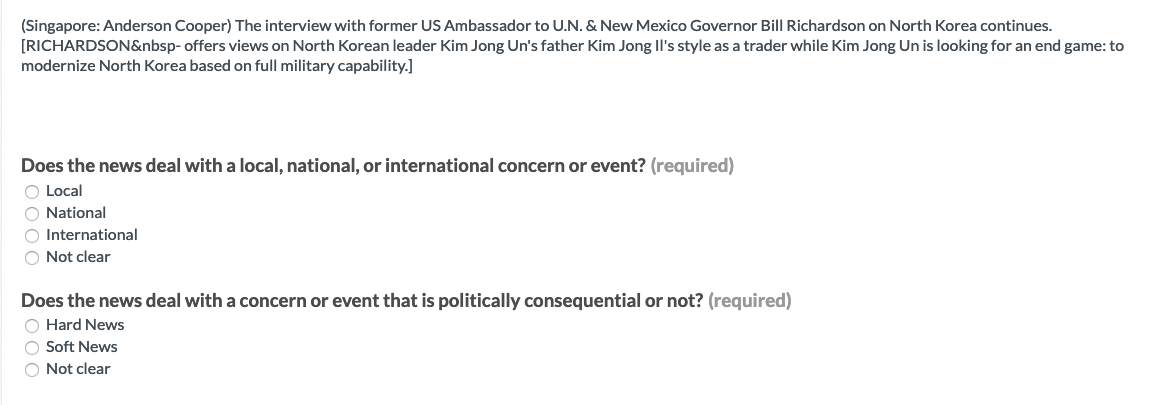
\includegraphics[width=\linewidth]{../data/screenshots/sample_question.png}
\end{figure}

\clearpage
\section{Supplementary Results}

\begin{figure}[H]
    \centering
    \caption{Proportion of Soft News by Channel}
    \label{fig:soft_over_time_by_channel}
    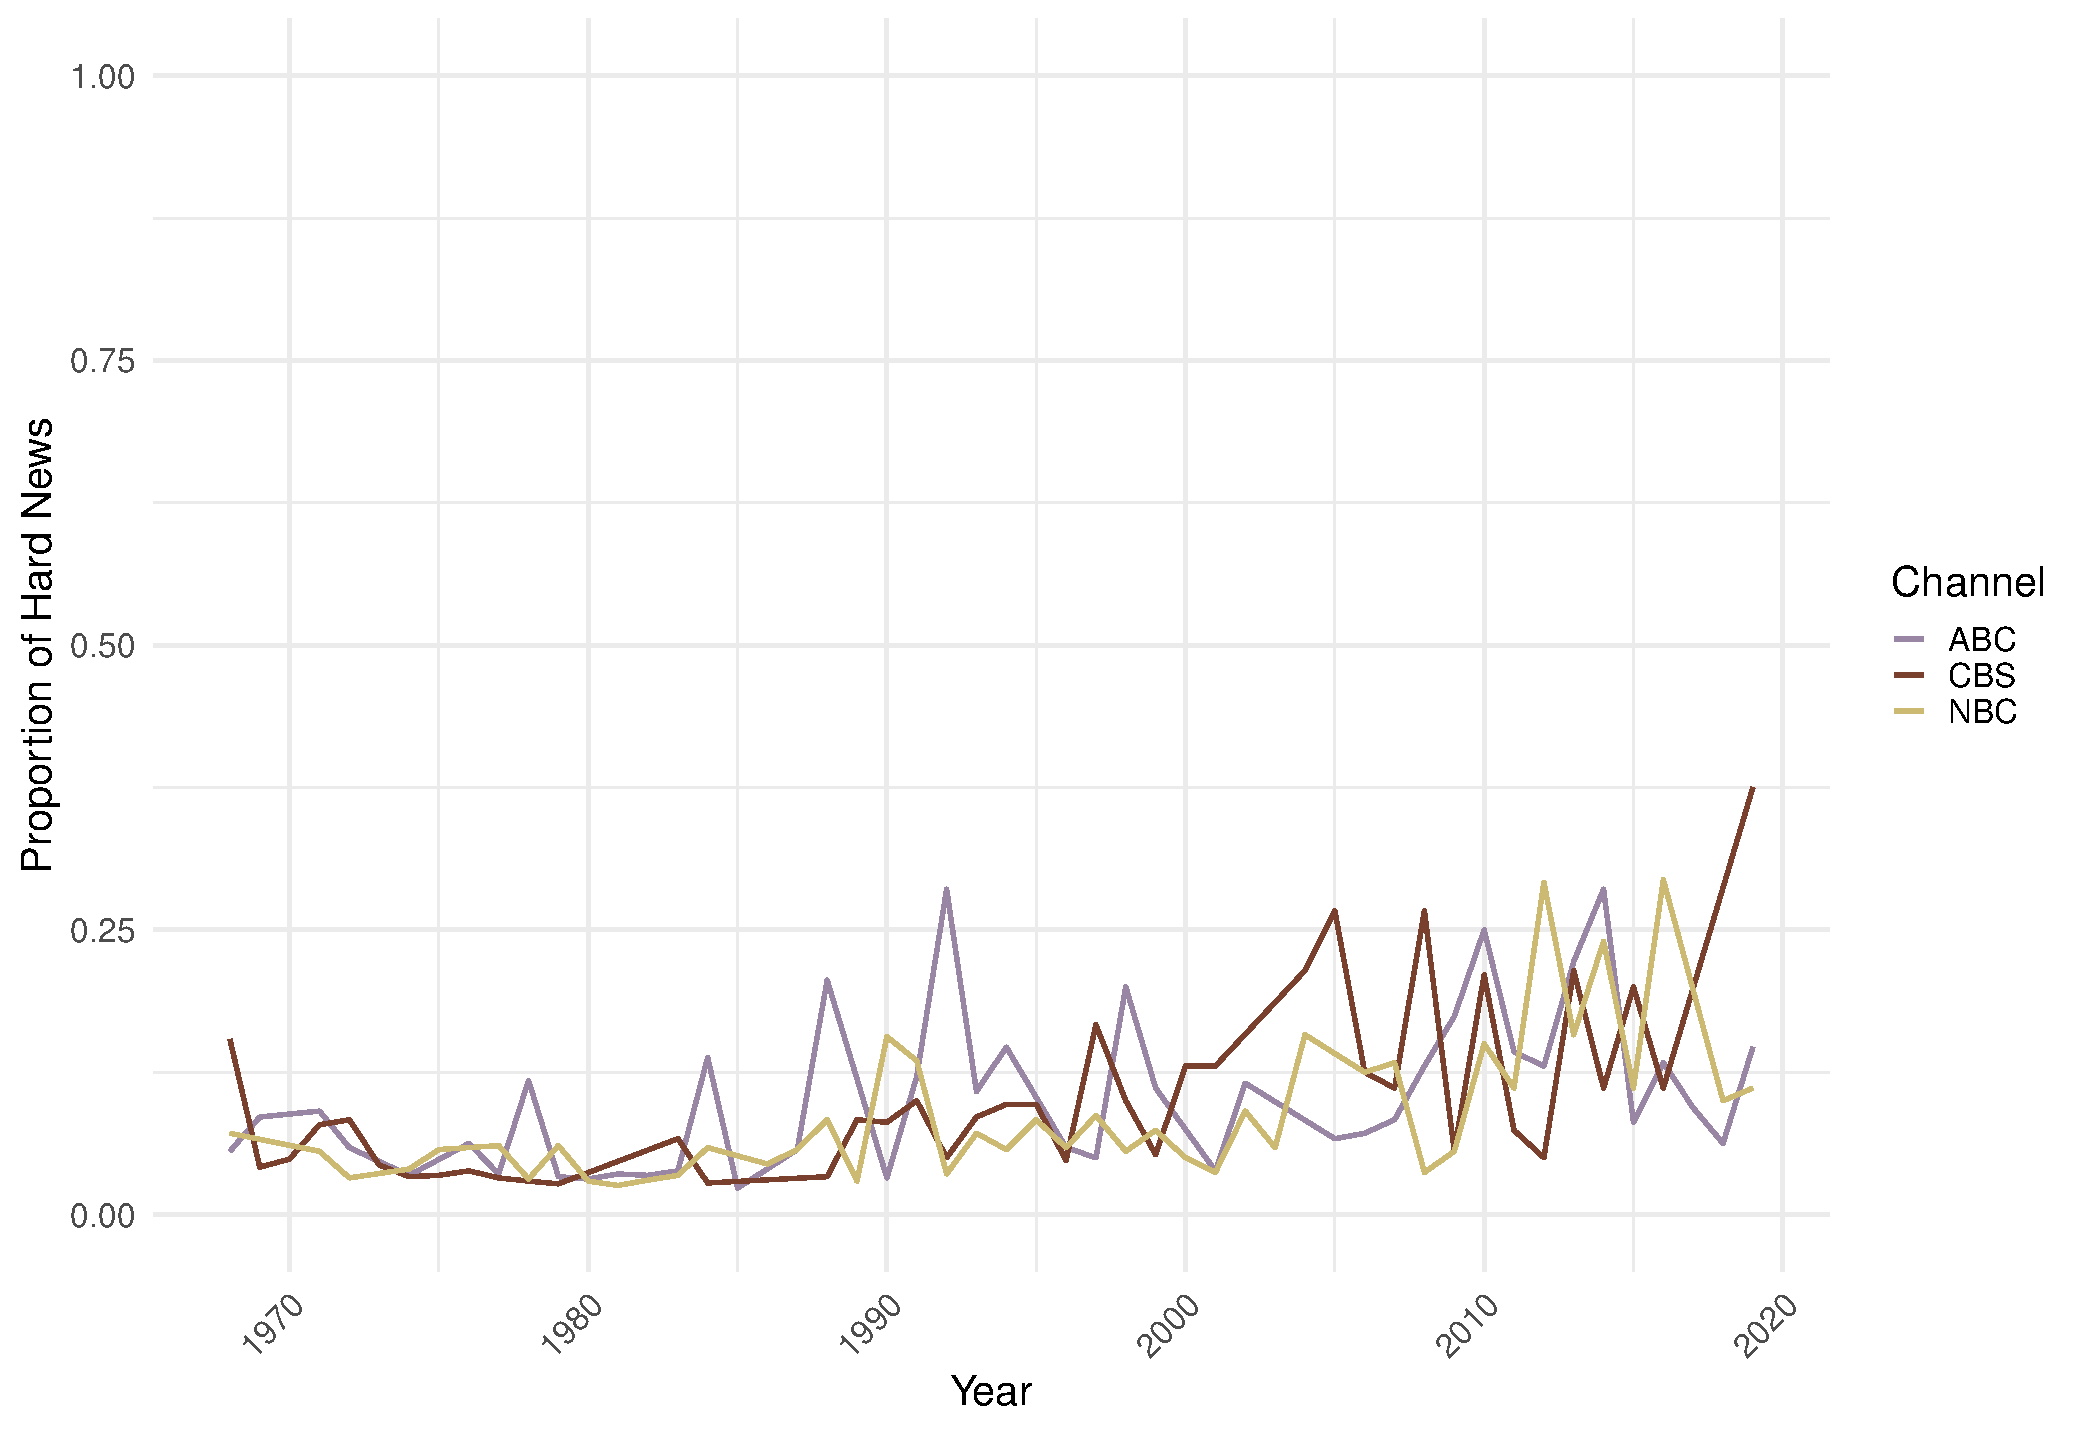
\includegraphics[width=.95\linewidth]{../figs/fig_prob_soft_channel.pdf}
\end{figure}


\begin{table}
\caption{Explaining The Provision of Different Types of News by Channel and Year (1970-2014)}
\begin{center}
\begin{tabular}{l c c c c }
\hline
 & Soft & International & National & Local \\
\hline
(Intercept)  & $0.08^{***}$ & $0.31^{***}$ & $0.59^{***}$  & $0.10^{***}$ \\
             & $(0.01)$     & $(0.01)$     & $(0.01)$      & $(0.01)$     \\
Channel: CBS & $-0.01$      & $-0.02$      & $0.03$        & $-0.01$      \\
             & $(0.01)$     & $(0.02)$     & $(0.02)$      & $(0.01)$     \\
Channel: NBC & $-0.01$      & $0.02$       & $-0.02$       & $-0.00$      \\
             & $(0.01)$     & $(0.02)$     & $(0.02)$      & $(0.01)$     \\
Year         & $0.04^{***}$ & $-0.00$      & $-0.05^{***}$ & $0.05^{***}$ \\
             & $(0.00)$     & $(0.01)$     & $(0.01)$      & $(0.00)$     \\
\hline
R$^2$        & 0.02         & 0.00         & 0.01          & 0.03         \\
Num. obs.    & 3923         & 3733         & 3733          & 3733         \\
\hline
\multicolumn{5}{l}{\scriptsize{$^{***}p<0.001$, $^{**}p<0.01$, $^*p<0.05$}}
\end{tabular}
\label{tab:news_over_time_7014}
\end{center}
\end{table}


\end{document}
